\documentclass{article}
\usepackage{fullpage}
\usepackage{setspace}
\usepackage[]{graphicx}
\usepackage[]{color}
\usepackage[OT1]{fontenc}
\usepackage{amsthm,amsmath,amsfonts}
\usepackage{natbib}
\usepackage[colorlinks,citecolor=blue,urlcolor=blue]{hyperref}
\usepackage{bm}
\usepackage{subcaption}
\usepackage{graphicx}
\usepackage{multirow}
\usepackage{xr}
\usepackage{tikz}
\usepackage{authblk}

%\usepackage{endfloat}

\doublespacing

\newcommand{\yti}{Y_{Ti}}
\newcommand{\yci}{Y_{Ci}}
\newcommand{\uti}{U_{Ti}}
\newcommand{\uci}{U_{Ci}}
\newcommand{\etat}{\eta(1)}
\newcommand{\etati}{\eta(1)_{i}}

\newcommand{\mti}{\bar{m}_{Ti}}
\newcommand{\byt}{\bm{Y_T}}
\newcommand{\byc}{\bm{Y_C}}
\newcommand{\bmt}{\bm{\bar{m}_T}}
\newcommand{\bmi}{\bm{m}_i}
\newcommand{\bsi}{\bm{s}_i}

\newcommand{\EE}{\mathbb{E}}

% see
% https://tex.stackexchange.com/questions/42726/align-but-show-one-equation-number-at-the-end
\newcommand\numberthis{\addtocounter{equation}{1}\tag{\theequation}}


\newenvironment{ass}[2][Assumption:]{\begin{trivlist}
\item[\hskip \labelsep {\bfseries #1}\hskip \labelsep {\bfseries #2}.]}{\end{trivlist}}

\def\independenT#1#2{\mathrel{\rlap{$#1#2$}\mkern2mu{#1#2}}}
\newcommand\independent{\protect\mathpalette{\protect\independenT}{\perp}}

\newcommand{\indicator}[1]{\mathbf{1}_{\left[ {#1} \right] }}






\title{Student Log-Data from a Randomized Evaluation of Educational
  Technology: A Causal Case Study}



\author[1]{Adam C Sales}
\author[2]{John F Pane}
\affil[1]{University of Texas, Austin, TX}
\affil[2]{RAND Corporation, Pittsburgh, PA}

%\affiliation{University of Texas College of Education and RAND Corporation}



\begin{document}
\maketitle

\section{Introduction}
In the 2007--2008 and 2008--2009 school years, the RAND corporation
conducted one of the first effectiveness trials awarded through
competitive grant programs sponsored by the US Department of
Education's Institute of Education Sciences.  The randomized
controlled trial (RCT) was
designed to estimate the effect of school-wide adoption of the
Cognitive Tutor Algebra I (CTA1) curriculum, whose centerpiece is a
computerized ``tutor'' that uses cognitive science principles to teach
Algebra I \citep{anderson1985intelligent}.
The study \citep{pane2014effectiveness} found no effects in its first year, but in
the second year of implementation students in schools randomized to
the CTA1 condition outperformed the control group on the posttest by a fifth of a
standard deviation.

Over the course of the CTA1 study, the software administrators
gathered computer log data for students in the treatment group.
They assembled a dataset that records which problems each student
worked, along with timestamps, the numbers of hints requested, and the
number of errors committed for each problem.
Log data from experiments like this present an unprecedented
opportunity for education researchers:
to use the fine-grained and rich data to
help understand how, why, and when educational technology works.

Along the same lines, log data presents a challenge, since it differs in
structure and size from the type of data commonly encountered in
studies of causal mechanisms.
While statistical models of log data are nearly as old as the data itself
\citep[e.g.][]{corbett1994knowledge}, data from an RCT differs in
two principal ways from more traditional domains.
RCTs feature randomization of treatment assignment, and a post-test
(or some other outcome) administered to both users and non-users.
These factors allow for causal modeling.

As educational technology booms, so do RCTs in the mold of the RAND
CTA1 study. A recent systematic review \citep{escueta2017education} cites 29
published reports of RCTs of ``computer assisted learning'' programs,
all but one of which was published since 2001. We are aware of
numerous other such RCTs planned or ongoing. The current case-study is
about the use of hints in CTA1, but the huge variation in products
under study, each with their own unique designs, opens a wide set of opportunities to understand how features of those
products drive their effects. As one example, RAND is currently
completing an efficacy study of a different algebra tutoring system,
ALEKS. When students begin working on a particular topic in ALEKS, the
system first presents instructional material, followed by problem
solving activities, and then, if students are unsuccessful at solving
the problems, more instructional material. Some students diligently
read the initial instructional material while others skip it and dive
directly into problem solving. Is skipping the material a productive
strategy for students in terms of learning algebra, or should ALEKS be
redesigned to prevent such skipping? Researchers should not stop at
estimating overall average treatment effects, but make use of the
wealth of log data that these RCTs produce automatically, as a
bi-product. Our hope is that this paper can serve as a starting point
for researchers interested in mining this rich resource.

The CTA1 effectiveness trial is a prominant example of a large and
growing number of randomized evaluations of educational technology
products (see \citealt{escueta2017education} for a recent systematic review).
In many, if not all, experimenters were able to
gather log data from students and/or teachers in the treatment group,
capturing the varying ways they used the technology.
These datasets could go a long way in helping researchers and
developers better understand how or for whom the software works.

This paper will illustrate three approaches to this type of research
using log data from the CTA1 study---specifically, data on students' use
of hints within the software.
The first approach discards the control group, and analyzes
hint-requesting in the treatment group as an observational study
\citep[c.f.][]{rosenbaum2002observational}. The
second approach applies the framework of causal mediation analysis
\citep{vanderweele2015explanation,hong2015causality,imai2011unpacking} to estimate the role of
hint-requesting in the overall CTA1 treatment effect. However, since
students in the control group were unable to request hints, not all
mediational estimands are identified, and estimation methods must be
modified.
Finally, we will conduct a principal stratification analysis
\citep{frangakis} to learn if students requesting different amounts of
hints experienced different treatment effects.

Our intention is to develop, demonstrate, and contrast these three
approaches to modeling log data.
We hope that this paper can serve as a starting point for
applied educational researchers interested in mining this rich
resource, and that this paper helps spur methodological interest in
this problem.
Ulitimately, we believe that education researchers should not stop at
estimating overall average treatment effects, but make use of the
wealth of log data that these RCTs produce.

After a brief overview of the three causal approaches we will discuss,
the next section will provide background for the case-study,
describing the CTA1 curriculum, the RAND study, and our focus on
hints.
The following three sections will present the observational study,
causal mediation, and principal stratification approaches to the hint
data.
Section \ref{sec:synthesis} will compare the three methods directly,
and discuss how they may be applied to data from other educational
technology RCTs.
Section \ref{sec:conclusion} will conclude.

\subsection{Brief Overview of Three Causal Approaches}
\begin{figure}
\centering
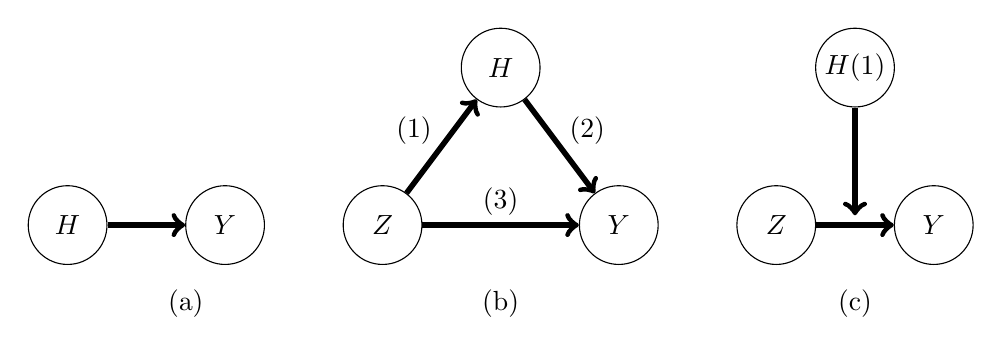
\begin{tikzpicture}[scale=1,transform shape]
	%\draw[help lines] (0,0) grid (15,3);
	\node[draw,shape=circle, inner sep=0pt,minimum size=1cm] (z) at (1,0) {$H$};
	\node[draw,shape=circle, inner sep=0pt,minimum size=1cm] (y) at +(0:3){$Y$};
	%\node[draw,shape=circle, inner sep=0pt,minimum size=1cm] (x) at (2.5,3.5){$X$};
	%\draw[->,line width=2pt](x)--(z);
	%\draw[->,line width=2pt](x)--(y);
	\draw[->,line width=2pt](z)--(y);
	\node at (2.5,-1) {(a)};

	\node[draw,shape=circle, inner sep=0pt,minimum size=1cm] (z) at (5,0) {$Z$};
	\node[draw,shape=circle, inner sep=0pt,minimum size=1cm] (y) at +(8,0){$Y$};
	\node[draw,shape=circle, inner sep=0pt,minimum size=1cm] (m) at (6.5,2){$H$};
	\draw[->,line width=2pt](z)--(m);
	\draw[->,line width=2pt](m)--(y);
	\draw[->,line width=2pt](z)--(y);
	\node at (5.4,1.2) {(1)};
	\node at (7.6,1.2) {(2)};
	\node at (6.5,.3) {(3)};
	\node at (6.5,-1) {(b)};

        \node[draw,shape=circle, inner sep=0pt,minimum size=1cm] (z) at (10,0) {$Z$};
	\node[draw,shape=circle, inner sep=0pt,minimum size=1cm] (y) at +(12,0){$Y$};
        \node (mid) at (11,0) {};
        \node[draw,shape=circle, inner sep=0pt,minimum size=1cm] (h)
        at (11,2) {$H(1)$};
	%\node[draw,shape=circle, inner sep=0pt,minimum size=1cm] (x) at (2.5,3.5){$X$};
	%\draw[->,line width=2pt](x)--(z);
	%\draw[->,line width=2pt](x)--(y);
	\draw[->,line width=2pt](z)--(y);
        \draw[->,line width=2pt](h)--(mid);
	\node at (11,-1) {(c)};

\end{tikzpicture}
\caption{A schematic representation of three causal models for
  log data: (a) an observational study estimating the effects of hints
  $H$ on posttest scores $Y$, (b) a mediation analysis estimating
  natural direct effects of treatment assignment $Z$ on $Y$ and
  indirect effects mediated by $H$, and (c) principal stratification.}
\label{mediationFig}
\end{figure}

Figure \ref{mediationFig} is a schematic representation of the three
approaches to causal modeling of log data that we will discuss in this
paper.
First, an observational study to estimate the effect of hint usage $H$
on posttest scores $Y$, is represented by figure (a).
This approach, which we will discuss in Section
\ref{sec:observational}, discards the control group from the RCT and
uses techniques from observational studies to determine if and how requesting
a greater number of hints affects post-test scores.
For the sake of illustration, we will use techniques similar to those
discussed in \citet{rosenbaum2002observational},
 \citet{hansen2009b}, and \citet{ho:etal:2007}, combining a propensity
 score matching design with methods for analyzing experiments and
 parametric modeling.
The conceptual and methodological issues we will discuss extend to
other covariate control methods as well.

Next, as represented in Figure (b), we will conduct a mediation analysis, estimating natural
indirect effects of CTA1 treatment assignment $Z$, as mediated by
$H$. That is, we will estimate the component of $Z$'s effect on $Y$ that comes about
due to $Z$'s effect on $H$---path (1)---and $H$'s effect on $Y$, path
(2).
Notice that path (2) is identical to figure (a)---the effect of $H$ on
$Y$.
We will use this equivalency to estimate and interpret indirect
effects.
As part of the mediation analysis, we will also estimate path (3), the
natural direct effect of $Z$ on $Y$---that is, the component of $Z$'s
effect on $Y$ that is not due to hints $H$.

Finally, we will estimate a principal stratification model, as represented in Figure
(c).
In the principal stratification analysis, we do not model $H$ as an
intervention that could, in theory, be randomized.
Instead, we posit a variable ``$H_i(1)$,''  subject $i$'s penchant for
requesting hints \emph{if} $i$ is assigned to the treatment
condition.
Unlike $H$, $H(1)$ is well defined (if
unobserved) for all participants in the RCT.
Principal stratification treats $H(1)$ as an effect moderator or
interaction variable: $H(1)$ does not affect $Y$, but the effect of
$Z$ on $Y$ may vary as a function of $H(1)$.
This analysis will largely follow the method of \citet{aoas}, which in
turn built heavily on \citet{schwartz2011bayesian} and
\citet{jin2008principal}.

All three of these approaches are designed to model intermediate
variables---those variables, like hint usage,
that were possibly affected by $Z$ but were measured prior to $Y$.
Though they were developed for more traditional data scenarios, the
novel scenario of computer log data from an educational technology RCT
presents new and interesting challenges and opportunities.

\section{Case Study: The Role of Hints in the Cognitive Tutor Effect}

\subsection{The Cognitive Tutor}
CTA1 is one of a series of complete mathematics curricula developed by
Carnegie Learning, Inc., which include both textbook materials and an
automated computer-based Cognitive Tutor
\citep{anderson1995cognitive,pane2014effectiveness}.

The computerized tutor was originally built to test the ACT and ACT-R
theories of skill acquisition \citep{anderson2013architecture}.
These are elaborate theories describing the necessary components of
cognitive skills in, say, mathematics or computer programming, and the
process of acquiring those skills.
The Algebra I tutor guides students through a sequence of Algebra I
problems nested in sections within units, and organized by the specific sets of skills they require.
Students move through the curriculum as the tutor's internal learning
model determines that they have mastered the requisite skills.

As students work through specific problems, they receive two types
of instruction from the tutor.
When they err---that is, depart from one of the pre-specified correct
solution paths for that problem---they receive an error message
alerting them to their mistake and helping them return to the correct
solution path.
Students may also request help, in the form of hints, that are also
tailored to the specific context and solution path of the problem.

\subsection{The Role of Hints}\footnote{This subsection draws heavily
  on comments from an anonymous reviewer.}
Students using the Cognitive Tutor Algebra software work algebra
problems on a computer, instead of on paper, as is typical.
But the Cognitive Tutor is not simply an online repository of
problems.
Each problem in the software is associated with a set of skills that
the student must master, and a path (or set of paths) to solving the
problem.
As soon as a student errs in working through the problem, the
software provides feedback tailored to the specific mistake, and
designed to guide the student back to a correct solution path.
Similarly, when a student gets stuck, and is unable to determine the
next step in solving the problem, he or she can ask for a hint.
Like the error feedback, these hints are tailored to the specific
algebra skills corresponding to the next step on the solution path.
Thus, hints and error feedback are crucial aspects of the tutor's
pedagogy.

On the other hand, the ready availability of hints may prevent some
students from trying to figure out algebra problems themselves,
instead asking for a hint as soon as things get hard.
If hints prevent student effort, they may be detrimental---after all,
students working through traditional worksheets or textbook problems
do not have recourse to hints and may put more effort into their
schoolwork.
\citet{koedinger2007exploring} refer to this as the ``assistance
dilemma.''

The RAND CTA1 effectiveness trial provides a valuable opportunity to
study the role of hints---on average, do they tend to help students
learn or to prevent them from learning?
What role does the availability of hints play in CTA1's effectiveness
when compared to traditional instruction?
Does requesting hints make CTA1 more effective or less?

\subsection{Data}\label{sec:data}

Since our goal was to better understand the CTA1
treatment effect, we focused our analysis on data from high school students in
the second year of the CTA1 trial, for whom the treatment effect was
most evident.

We merged data from two sources: covariate, treatment and outcome data gathered by RAND, and computerized log data gathered by Carnegie Learning.
Table \ref{tab:covariateBalance} describes the covariates we used, including
missingness information, control and treatment means, and standardized
differences \citep[c.f.][]{kalton1968standardization}.
We singly-imputed missing values with the Random Forest routine implemented
by the \texttt{missForest} package in \texttt{R}
\citep{missForest,rcite},  which estimated the ``out of box'' imputation
errors also shown in Table \ref{tab:covariateBalance} as part of the random forest regression.

\begin{table}[ht]
\centering
\include{output/covariateTable}
\caption{Missingness information and balance for the covariates included in this study, from
  the CTA1 Effectiveness experiment, high
  school, year two. Imputation error is percent falsely classified for
  categorical variables (Race/Ethnicity, Sex, and Special Education)
  and standardized root mean squared error for Pretest, which is
  continuous. %The overall p-value accounts for clustering at the
  %school level and blocked random sampling.
  Analysis done in \texttt{R} via \texttt{RItools} \citep{ritools}.}
\label{tab:covariateBalance}
\end{table}


Over the course of the effectiveness study, Carnegie Learning gathered
log data for each worked problem.
The resulting dataset lists the problem name, section, and unit of
each problem, the numbers of hints requested and errors committed, and time-stamps.
Log data were missing for some students, either because the log files were not retrievable, or because of an imperfect ability to link log data to other student records.
Treatment schools with mastery data missing
for 90\% or more students were omitted from the analysis, along with
their entire randomization block.
Of the remaining 2,390 students, 87\% (2,091) had log
data.
The students with missing log data were dropped from the observational
study and mediation analysis, but included in the principal
stratification study.
Problem log data for sections that were not part of the
standard CTA1 Algebra I curriculum and problems worked by fewer than 100
students were omitted from the
dataset.

All told, the main analysis included $n=$5308 students, 2390 of whom were assigned to the CTA1 condition and 2918 of whom were assigned to control.
The students were nested within 116 teachers, in 43 schools across five states.


\section{Measuring Hint Requests}\label{sec:modelingHints}
In our CTA1 log data, 2091 students requested a total of 801,518 hints on
926,314 problems.
Some students never requested a hint, and one student requested over
three thousand hints; some students requested at least one hint on every problem
they worked.

Clearly, several factors played a role in this variation.
First, academically weaker students---those whom we would expect to
score lower on the posttest regardless of CTA1 use---probably struggle
with CTA1 problems more often, and probably request more hints.
This presents a serious confounding threat, which we will attempt to
address in a number of ways throughout the paper.
Our first line of defense is a slight restructuring of the causal
questions, reflected in the measurement stage.
By ``hint use'' we refer to a student's use of hints on problems that
he or she finds challenging.
Specifically, we consider only worked problems on which
the student either requested a hint or committed an error.
This effectively filters out the problems that each student finds
trivial; the fact that stronger students struggle less often is no
longer a driving factor.
(In an equivalent formulation, the question addresses each student's
likelihood of committing an error without having asked for a
hint---i.e. deciding to attempt a difficult problem without help.)
This strategy removes some of the confounding between
student ability and hint requests, though (as we shall see) a
substantial amount remains.

Factors beyond student ability also play a role in the variation
in the numbers of hints students requested.
For one, students who worked a larger number of CTA1 problems also
requested more hints.
Secondly, not all problems are equivalent.
Problems vary in their structure, and hence in the number of hints
available---some problems allow an indefinite number of hint requests.
Problems from some sections never elicited hints, whereas problems
from other sections nearly always did.
A students' hint requests are a function of their learning
style within the tutoring software, which parts of the software they
worked, and how much they worked.

A focus on hint requests, as opposed to these other
factors, requires some care.
Modeling hint requests per problem as binary---did a student request
at least one hint?---puts problems with many or few
available hints on equal footing.
Problem difficulty is another matter.
What is difficult for one student may not be difficult for others.
That students do not request hints on problems they find trivial is
uninteresting; what is more interesting is how they react when a
problem presents a challenge.

\begin{figure}
\centering
\includegraphics[width=0.95\textwidth]{rasch.jpg}
\caption{The proportion of problems in which each student requested a
  hint, or the IRT student parameter $\eta$ from model
  (\ref{eq:rasch}), as a function of each student's average section difficulty. For each
  section, ``section difficulty'' is defined as the proportion of
  \emph{that section's} worked problems that elicited a hint request,
  and a student's average section difficulty is the average section
  difficulty over that student's worked problems.}
\label{fig:mbar}
\end{figure}

To capture the effect of hint requesting behavior, as distinct from
total amount of usage, a first step may be to calculate the proportion
of each student's challenging problems that resulted in a hint
request.
However, this presents additional issues, one of which can be seen in Figure
\ref{fig:mbar}.
First, even after dichotomizing hints and restricting our focus to
instances in which students appear to be challenged, worked problems
may differ from each other in relevant ways.
For instance, multi-step problems which provide more occasions for hint
requests may elicit at least one hint more frequently.
For each section of the tutor, let ``section difficulty'' be the proportion of that
section's challenging problems that elicited a hint request; let a
student's ``average section difficulty'' be the average section
difficulty over all challenging problems that student worked.
On the left of Figure \ref{fig:mbar}, the proportion of problems on
which each student requested at least one hint is plotted against that
student's average section difficulty.
It is apparent, if unsurprising, that students who worked on sections of the
curriculum that typically elicited more hints tended to request hints
more often.
The Spearman correlation between average section difficulty and hint
request proportion is 0.35.
How do we equate the hint records of students who worked problems in different
sections?

% Further, hint request proportions are related to the number of
% challenging problems each student worked, as can be seen on the right
% panel of Figure \ref{fig:mbar}.
% This is due to measurement error.
% The variance of a sample proportion is inversely proportional to the
% size of the sample; therefore, it is unsurprising that the extremes of
% hint request proportions are composed primarily of students who worked
% very few problems.
% For instance, nearly all students who requested a hint on more than
% 75\% of the problems that challenged them worked fewer than 250
% challenging problems.

Item response theory \citep[e.g.][]{irtHandbook} provides an attractive alternative.
Under a modified Rasch model \citep[e.g.][]{rasch}, for instance,
\begin{equation}\label{eq:rasch}
Pr(h_{ip})=logit^{-1}(\eta_i+\delta_{s[p]})
\end{equation}
where $h_{ip}$ is the event that student $i$ requests a hint on
problem $p$, $\eta_i$ is a student parameter, $\delta_{s[p]}$ is a
section-level parameter for $s[p]$, the section that problem $p$ was
drawn from, and $logit^{-1}(x)=\{1+exp(-x)\}^{-1}$ is the inverse logit
function.
Typically, the student parameter $\eta_i$ measures student ability;
here, instead, it measures a student's proclivity to request a hint.
The typical Rasch model includes a problem-level ``difficulty'' parameter, but in our
dataset many problems were worked by very few students, so problem
level parameters would be hard to estimate.
Instead, we included the section-level parameter $\delta_{s[p]}$,
which measures the extent to which students tend to request hints on
problems in section $s$.
This essentially assumes that all problems in each section are equally
likely to elicit a hint.
Replacing student hint request proportions with the posterior mode for
$\eta$ from model (\ref{eq:rasch}), fit using the \texttt{lme4}
package in \texttt{R} \citep{lme4}, resolves the section-difficulty conundrum: the right
side of Figure \ref{fig:mbar}, in which $\eta$ is plotted instead of
hint request proportion, shows no substantial relationship between
section difficulty and hint requests.

In some analyses, we dichotomize $\eta$ with a median split.
Let $H_i=1$ if $\eta_i>median(\bm{\eta})$ and 0 otherwise.
While in dichotomizing $\eta$ we lose valuable information, doing so
simplifies the observational matching design of the following section,
and makes the mediation analysis possible.


\section{An Observational Study Within an Experiment}\label{sec:observational}

How does requesting hints within CTA1 affect learning?
More precisely, would students have achieved higher posttest scores
had they requested hints more (or less) often?

Let $Y_i$ represent subject $i$'s posttest score, and let $Z_i$ represent
$i$'s treatment status (i.e. the CTA1 or control group).
Following \citet{neyman} and \citet{rubin}, let $Y_i(Z=1)$ be
the posttest score student $i$ would exhibit were $i$ (perhaps
counterfactually) assigned to the treatment condition, and
$Y_i(Z=0)$ the score were $i$ assigned to control.
Then the CTA1 treatment effect for student $i$ is $Y_i(Z=1)-Y_i(Z=0)$.
A similar structure applies to hint request for students in the
treatment group.
For these students, let the potential outcomes be $Y_i(Z=1,H=1)$ and
$Y_i(Z=1,H=0)$ or $Y_i(H=1)$ and $Y_i(H=0)$ for short.
For a study measuring hint requests as a continuous variable, we may
define $Y_i(\eta)$, the posttest score $i$ would exhibit were $i$ to
request hints with proclivity $\eta$.
This structure implicitly assumes ``non-interference,'' that one
student's treatment assignment $Z$ or hint proclivity $H$ does not
affect another student's posttest scores.

Individual treatment effects are (typically) unidentified, since only
one of the relevant potential outcomes is ever observed for each
subject.
For instance, $Y(H=1)$ is unobserved for members of the
treatment group with $H=0$.
If $Pr(H_i=1)$ were known for each $i$ (as would be the case if $H$
were randomized) then the average treatment effect (ATE) of $H$ on $Y$,
$\EE[Y(H=1)]-\EE[Y(H=0)]$, could be estimated without bias or further
assumptions.
Of course, the distribution of $H_i$ is unknown, and is presumeably a
function of $i$'s individual characteristics.
However, if these relevant characteristics were all measured and
available, the ATE of $H$ on $Y$ would be identified.

Let $\bm{x}_i$ represent a vector of baseline covariates for subject $i$.
In our study of hints, $\bm{x}$ includes indicators for state, school
id, class id, grade (9th or higher), race (White/Asian,
Black/Multi-Racial, or Hispanic/American Indian/Alaskan Native),
special education status, economic disadvantage, and English language
learner status, as well as pre-test scores.
Then we assume \citep[c.f.][]{rosenbaum1983central}:
\begin{ass}{Strong Ignorability}
\begin{equation*}
 \{Y(H=1),Y(H=0)\}\independent H |\bm{x}
\end{equation*}
\end{ass}
that conditional on $\bm{x}$, potential outcomes $Y(H=1)$ and $Y(H=0)$
are independent of realized $H$.
Under strong ignorability, one may compare subjects with identical
covariates $\bm{x}$ to estimate causal effects.

Unfortunately, this sort of exact matching is impossible in our finite
sample.
Instead, we estimated ``propensity scores'' \citep{rosenbaum1983central}:
\begin{equation*}
\pi_i=Pr(H_i=1|\bm{x})
\end{equation*}
the probability of a treatment-group subject requesting frequent hints, conditional on
his or her covariate vector $\bm{x}$.
\citet{rosenbaum1983central} shows that conditioning on $\pi$ is
equivalent to conditioning on $\bm{x}$.
We estimated $\pi$ using a Bayesian multilevel logistic regression,
with weakly informative priors, using the \texttt{rstanarm} package in
\texttt{R} \citep{rstanarm}.
The propensity score model was:
\begin{equation*}
\pi_i=logit^{-1}(\alpha+\bm{\tilde{x}}\bm{\beta}+\epsilon^{state}+\epsilon^{school}+\epsilon^{class})
\end{equation*}
where $\bm{\tilde{x}}$ is the $\bm{x}$ vector excluding indicators for
state, school, and class, which were each included using random
intercepts modeled as normally distributed.

We constructed an optimal full matching design \citep{hansen2004} to
condition on estimated propensity scores $\hat{\pi}$ using the
\texttt{optmatch} package in \texttt{R} \citep{optmatch}.
We matched $H=0$ subjects to $H=1$ subjects in such a way as
to minimize the overall distance between subjects in matched sets in
the logit-transformed propensity scores, $logit(\hat{\pi})$.
We constrained the match so that students could only be matched within
schools.
This was for two reasons: first, schools determine a number of factors
that in turn may impact posttest scores, including baseline
student characteristics, pedagogical styles, and CTA1 usage patterns
\citep[see][]{descriptivePaper}, and second, doing so facilitated the mediation
analysis in the following section.
Each matched set was allowed to contain any positive number of $H=1$
and any positive number of $H=0$ subjects, resulting in matches of
variable size and composition.
For instance, one matched set included 30 $H=1$ subjects matched to a
single $H=0$ subject, and another matched 21 $H=0$ subjects to a
single $H=1$ subject.

Table \ref{fig:balance} in the online appendix shows that
matching largely eliminated mean differences in pre-treatment
covariates between $H=1$ and $H=0$ students.
The only notable exception is in pretest scores: $H=1$ students tended
to have slightly higher pretest scores than their matched comparisons
with $H=0$.
The p-value from an omnibus covariate balance test
\citep{covBal} is 0.26.

Let $m_i$ be a categorical variable denoting the matched set that $i$
belongs to.
Then we may re-state the ignorability condition with reference to this
match \citep[c.f.][]{rebar}:
\begin{ass}{Matched Ignorability}
\begin{equation*}
 \{Y(H=1),Y(H=0)\}\independent H |m
\end{equation*}
\end{ass}
% Matched ignorability formalizes a ``latent experiment'' design: by
% assuming matched ignorability, we imagine a randomized trial in which
% members of the CTA1 group were divided into strata defined by $m$, and
% randomized to $H=1$ or $H=0$ within those strata.
Under matched ignorability, the mean of the outcomes between $H=1$ and
$H=0$ students within each match is unbiased for the average treatment
effect for students in that match.
The (weighted) mean of those estimated treatment effects estimates the
overall treatment effect in the sample.

% The classic approach to estimating effects from blocked randomization
% designs is a fixed-effects regression \citep{fisher1926arrangement},
% regressing outcomes on an indicator for treatment assignment and a set
% of indicators for matched sets.
% The results from this analysis are displayed on the row labeled
% ``ANCOVA'' in Table \ref{tab:matchResults}, with ``HC3'' standard
% errors and 95\% confidence intervals.
% They suggest that a greater-than-median proclivity to request hints
% \emph{hurts} student learning by a large amount, roughly equal to the
% entire treatment effect of CTA1 estimated in
% \citet{pane2014effectiveness}.
Table \ref{tab:matchResults} gives three treatment effect estimates
under matched ignorability.
The rows labeled ATE and TOT weight the matched sets to
estimate the average effect of $H$ over the entire treatment
group and over those members of the treatment group with $H=1$,
respectively.
The row labeled ANCOVA of Table \ref{tab:matchResults} gives the
coefficient on $H$ from a regression of Y on $H$ along with indicators for matched set,
racial categories, grade, ESL status, economic disadvantage, and sex,
along with linear and quadratic terms for pre-test (the standard error
and confidence interval use the ``HC3'' sandwich estimator,
\citealt{sandwichPackage}).
This regression adjusts for imbalances in these covariates within
matched sets \citep[c.f.][]{biasAdjust}; its estimate is similar to
the others.


\begin{table}
\centering
\begin{tabular}{crllcll}
&&Est.&SE&95\% CI&$\rho^2$&$T_Z$\\
\hline
\multirow{4}{*}{Estimate}%&ANOVA& -0.22 &0.04 &[-0.30,-0.13]&0&0\\
&ATE&-0.24&0.05&[-0.33,-0.14]&0&0\\
&TOT&-0.21&0.06&[-0.33,-0.10]&0&0\\
&ANCOVA&-0.22&0.04&[-0.31,-0.14]&0&0\\
\hline
\multirow{2}{*}{Sensitivity}&[Pretest]&-0.22&&[-0.55,0.10]&0.17&-13.14\\
&[Pretest/2]&-0.22&&[-0.40,-0.05]&0.08&-6.57\\
\hline
\end{tabular}
\caption{Estimates with and without regression adjustment and
  sensitivity analysis of the effect of hint usage.}
\label{tab:matchResults}
\end{table}

Matched ignorability is a very strong assumption, so these results
should not be taken at face value---especially if weaker students ask for hints at
higher rates, and also score lower on the posttest.
While adjusting for pre-test scores via matching and/or regression
may account for some of that bias, pre-test may not capture all of the
relevant pre-treatment information.
To account for the possibility of unmeasured confounding, we conducted
a sensitivity analysis following the method of \citet{hhh}.
This method imagines a hypothetical missing covariate $U$ and estimates
how the the omission of $U$ alters the estimate
and its standard error.
The result is a ``sensitivity interval'' \citep[c.f.][]{rosenbaum2002observational} that,
with 95\% confidence, contains the true effect accounting for both
sampling uncertainty and uncertainty due to possible confounding.
$U$ is characterized by two sensitivity parameters:
$\rho^2$ is the squared partial correlation between $U$ and $Y$, after
accounting for the observed covariates in the model, and $T_Z$ is the
t-statistic from an ordinary least squares regression of $H$ on $U$, along with the observed covariates.
These sensitivity parameters may be benchmarked by estimating their
counterparts when observed covariates are left out of the model.
The row of Table \ref{tab:matchResults} labeled ``[Pretest]''
imagines a $U$ that predicts $Y$ and $H$ to a similar extent as
pretest.
The resulting sensitivity interval is quite wide, including
unbelievably large negative effects as well as substantial positive
effects.
A slightly less conservative sensitivity analysis, labeled
``[Pretest/2]'' allows $U$ to
predict $H$ and $\rho$ half as well as pretest scores.
This sensitivity interval is wide, but entirely negative.

\subsection{The Observational Study Approach: Interpretation and Discussion}
The observational study approach to log data seeks to estimate the
effect of a usage parameter, estimated from  computer log data, on
outcomes.
This approach does not exploit randomization---in fact, it discards
the control group entirely.
However, it depends heavily on another feature of RCTs: namely, an
outcome measured for all participants, in this case a posttest.
Causal identification derives not from randomization, but from an
untestable ignorability assumption, coupled with a sensitivity analysis.
In our example, we operationalized strong ignorability with a
propensity-score matching design, but other observational study
designs may apply as well.

We found that hint requests have a negative effect: students who tend
to request hints more often than the median score lower on the
posttest, after controlling for observed covariates.
When hint usage is expressed numerically, we find a monotonically
decreasing relationship between hint requests and posttest scores---as
far as we can tell, the optimal strategy is to never request a hint.
However, this observed effect may be due to confounding.
If, say, weaker students ask for hints more often and score lower
on the posttest regardless of hint usage, posttest scores will be
anticorrelated with hint requests.
This could even be the case after control for pretest scores and other
covariates, if these failed to capture all of the relevant dimensions
of student ability.
We found that an unobserved confounder that predicts both hint usage
and posttest scores just as strongly as the pretest could explain the
entire observed relationship.
The data, coupled with the existence of such a missing covariate, are
consistent with both positive and negative effects of hint requests.
On the other hand, covariates that are as important as pretests are
quite rare in practice---this confounding scenario might not be
plausible after all.
A less extreme missing confounder, predicting $Y$ and $H$ with half
the strength of the pretest, cannot explain the observed relationship,
and is only consistent with negative effects of hint requests.

Despite being hobbled by the lack of randomization, and the resultant
threat of confounding, the observational study approach provides weak
evidence that hints are harmful to posttest scores---a potentially
important finding.
This result, if confirmed in other scenarios and other analyses, may
inform student behavior in the tutor and future tutor designs.
However, since it ignores the control group from the CTA1 RCT, it does
not shed light on the CTA1 causal mechanisms---it does not explain the
CTA1 effect.
However, its design and results figure prominently in mediation
analysis, which does.

\section{Mediation Analysis}\label{sec:mediation}
The goal of causal mediation analysis is to decompose a treatment
effect into an ``indirect'' or ``mediated''
effect and a ``direct'' effect.
The indirect effect captures the component of the effect that is due
to the mediator: the treatment affected the outcome by affecting the
mediator, which itself, in turn, affected the outcome.
In contrast, the direct effect is the component of the effect that
operates via other mechanisms.

More precisely, express a subject's potential outcomes as a function
of two variables, treatment assignment $Z$ and hint requests $H$:
$Y(Z,H)$.
Now, if $Z$ and $H$ are both binary, as in our example, subjects
each have four potential outcomes:
\begin{equation*}
Y(0,0);\;Y(1,0);\;Y(0,1);\;Y(1,1)
\end{equation*}
representing the outcomes they would exhibit were they assigned to
control and requested few hints, assigned to
treatment and requested few hints, assigned to control and requested
many hints, or assigned to treatment and requested many hints.
In the CTA1 trial, however, the potential outcome $Y(0,1)$ is
meaningless: students in the control group had no access to CTA1, and
therefore could not request hints.
This will be an important factor going forward.

Since $H$ is itself affected by treatment assignment, it
too has potential values:
\begin{equation*}
H(0);\;H(1)
\end{equation*}
representing the hints that would be requested under treatment and
control.
In the CTA1 study, $H(0)=0$ for all subjects.

Combining potential values for $Y$ and for $H$ yields the fundamental
building blocks of causal mediation analysis
\citep[e.g.][]{vanderweele2015explanation,sales2017mediation}.
Let $Y(z,H(z'))$
represent the outcome that a subject would express given treatment
assignment $z$, but the hint behavior that he or she would have
expressed under assignment $z'$.
When $z=z'$, the original two potential outcomes for $Y$ emerge:
$Y(1,H(1))=Y(Z=1)$ is the outcome exhibited under the treatment, when $H$
takes its potential treatment value; similarly, $Y(0,H(0))=Y(Z=0)$. On
the other hand, $Y(1,H(0))$ and $Y(0,H(1))$ are strictly
counterfactual. $Y(1,H(0))$ gives the outcome value
that would result for a subject assigned to the treatment condition
but who nevertheless requested hints as he or she would have under
control. $Y(0,H(1))$ gives the potential outcome for a subject
assigned to control but who nevertheless requested hints as he or she
would have under treatment.
This last quantity is problematic in our case, since $H(1)$ can take the value 1,
and as we have seen $Y(0,1)$ is undefined.

This framework facilitates precise definitions of direct and indirect
effects; in fact, there are two versions of each \cite[e.g.][]{imai2011unpacking}:
\begin{align*}
\delta(1)&=Y(1,H(1))-Y(1,H(0))\\
\delta(0)&=Y(0,H(1))-Y(0,H(0))\\
\end{align*}
are the indirect effects, contrasting potential outcomes when $H$
varies as it would with varying treatment assignment, but holding the
assignment itself constant at either 1 or 0.
\begin{align*}
\xi(1)&=Y(1,H(1))-Y(0,H(1))\\
\xi(0)&=Y(1,H(0))-Y(0,H(0))\\
\end{align*}
represent the direct effects: holding the value of $H$ constant,
either at its potential value under treatment or control, while
varying treatment assignment.
The total treatment effect, $Y(1,H(1))-Y(0,H(0))$, can then be
decomposed in two ways: as $\delta(1)+\xi(0)$ or as
$\delta(0)+\xi(1)$.
These decompositions can potentially reveal the role hints play in the
CTA1 treatment effect: $\delta(1)$ gives the extent to which
assignment to CTA1 affects a student's post-test score by (possibly)
causing him or her to request hints.
$\xi(0)$ gives the effect of assignment to CTA1 if hints were,
perhaps counterfactually, held at their control level, $H=0$.


\subsection{Identification and Estimation of Direct and Indirect
  Effects}

Since the potential outcome $Y(0,1)$ is undefined in the CTA1 hints
study, any expression (potentially) including $Y(0,1)$ is also
undefined; this includes $\delta(0)$ and $\xi(1)$.
Indeed, since hint behavior is unobserved in the control group
altogether, conventional approaches to mediation analysis do not
apply.
Further, were we to operationalize hint behavior as a continuous
variable, as may seem natural, mediation analysis in this case would
also be nearly impossible.
This is because students assigned to the control group request exactly
zero hints, whereas merely nine members of the treatment group
requested no hints over the course of the study, and these students
barely used the tutor at all.
That being the case, the data provide little to no information about
the distribution of potential outcomes when the software is used
but no hints are requested.

Our solution was to dichotomize hint requests with a median split, as
described above, essentially re-defining the causal question.
Half of the treatment group and all of the control group has
$H=0$---requesting hints at a rate less than the (treatment group)
median.
To make sense of the respective roles of $H$ and $\eta$, the
continuous measure on which it is based, we may imagine a process in
which students are assigned $H$, and under that constraint choose a
value for $\eta$.
In the control group all students are assigned $H=0$ and $\eta=0$, but
in the treatment group half of students have $H=1$ and half have
$H=0$, and $\eta$ varies within those groups.
That structure implies a ``treatment mediator interaction''
where the effect of the mediator on the outcome varies by treatment
status.
Of course, in our example treatment mediator interactions are not
identified, since $H=0$ and $\eta=0$ in the control group, and very
few treatment students asked for 0 hints.
In any event, dichotomizing hint requests likely undersells the role
of hints, but allows a tractable mediation analysis.

In principle, effects $\delta(1)$ and $\xi(0)$ are defined at the
individual level, as $\delta(1)_i$ and $\xi(0)_i$.
However, as in the usual causal inference case, individual effects are
not identified without strong assumptions, and the target of
estimation is instead taken to be super-population average effects,
$\EE[\delta(1)]$ and $\EE[\xi(0)]$. Our approach to estimating these
is to estimate the means of each of the component potential outcomes,
$\EE Y(1,H(1))$, $\EE Y(1,H(0))$, and $\EE Y(0,H(0))$.
The first and last of these, $\EE Y(1,H(1))=\EE Y(Z=1)$ and $\EE
Y(0,H(0))=Y(Z=0)$ are non-parametrically identified due to the
randomization of treatment assignment.

On the other hand, randomization alone does not identify the strictly counterfactual
potential outcome $\EE Y(1,H(0))$.
In a typical mediation analysis of an RCT, identification of the
distribution of $H(0)$ in the population would derive from
randomization, along with an observation of $H$ in the control group.
In contrast, in the CTA1 study, $H(0)$ is not observed but is
determined by the experimental design: since the CTA1 software was
unavailable to the control group, $H(0)=0$ for all experimental
participants.
Therefore, $Y(1,H(0))\equiv Y(1,0)$.
For treated subjects $i$ for whom $H_i=0$, then, $Y_i(1,H(0))=Y_i$,
the observed outcome is equal to the counterfactual outcome.
For these subjects, there is no indirect effect.

Treated subjects with $H=1$ present more of a challenge.
To estimate indirect effects for these subjects, we may rely on the
same causal setup as in the observational approach:
matched ignorability and the matching design of section
\ref{sec:observational}.
If $Y_i(1,H(0))$ is independent of $Z_i$ within matched sets, then we
may estimate counterfactual potential outcomes for $H=1$ subjects
using the observed outcomes of their matches with $H=0$.
Specifically, let
\begin{equation*}
\hat{Y}_i(1,H(0))=\begin{cases}
 Y_i & H_i=0\\[3ex]
\frac{\displaystyle\sum_{j:M_j=M_i}
  Y_j(1-H_j)}{\displaystyle\sum_{j:M_j=M_i} 1-H_j} & H_i=1
\end{cases}
\end{equation*}
For treated subjects with $H=1$, the estimated $\hat{Y}(1,0)$ is the
average outcome of their matched pairs with $H=0$.
Then, the average indirect effect in the treatment group can be
estimated as:
\begin{equation*}
 \hat{\Delta}\equiv\widehat{\EE[\delta(0)|Z=1]}=\frac{1}{n_T}\displaystyle\sum_{i:Z_i=1} Y_i-\hat{Y}_i(1,H(0))
\end{equation*}
(Typically, the overall average indirect effect, $\EE[\delta(0)]$, is
estimated instead of the average indirect effect of the treatment
group, $\EE[\delta(0)|Z=1]$.
We estimated the latter since data from the control group was not used
in our estimation strategy, and estimating the overall average would
simply complicate our standard error estimation.)

This estimate is a close cousin of the ``TOT'' estimate in Table
\ref{tab:matchResults} from the previous section.
Recall that the TOT effect is the average effect of $H$ on treatment
group subjects with $H=1$.
Both estimate contrast outcomes between $H=0$ and $H=1$, and both use
data from only the treatment group.
TOT is the the difference between the average outcome for students in
the treatment group with $H=1$, and the average outcome under the
counterfactual scenario in which they all had $H=0$.
That is,
\begin{equation*}
TOT=\EE[Y(1,1)|Z=1,H=1]-\EE[Y(1,0)|Z=1,H=1]
\end{equation*}
$\hat{\Delta}$ estimates the difference between the average outcome
for students in the entire treatment group, and the average outcome
for the treatment group were $H=0$ for all students.
That is
\begin{equation*}
\Delta=\EE[Y(1)|Z=1]-\EE[Y(1,0)|Z=1]
\end{equation*}
This can be re-written (omitting conditioning on $Z$):
\begin{align*}
\begin{split}
\Delta&=\EE[Y(1,1)|H=1]Pr(H=1)+\EE[Y(1,0)|H=0]Pr(H=0)\\
&\qquad -\EE[Y(1,0)|H=1]Pr(H=1)-\EE[Y(1,0)|H=0]Pr(H=0)
\end{split}
\\[2ex]
&=(\EE[Y(1,1)|H=1]-\EE[Y(1,0)|H=1])Pr(H=1)
\end{align*}
Since $Pr(H=1)=1/2$ ($H$ was defined with a median split),
$\hat{\Delta}=TOT/2$.
Estimated thusly, the indirect effect is negative: $-0.11$, with
a standard error of 0.03.
This analysis suggests that the availability of excessive hints
actually \emph{lowers} the treatment effect.
CTA1 works not because of hints, but despite them.

What would the effect be without hints?
To answer that question, we estimate ``direct'' effects,
$\Xi=\EE[\xi(1)]=\EE[Y(1,H(0))]-\EE[Y(0,H(0))]$.
Like indirect effects, this expression includes the average potential
outcome $\EE[Y(1,H(0))]$; unlike indirect effects, includes a term for
potential outcomes under the control condition.
Since the main contrast of $\Xi$ is due to treatment assignment,
construction of the estimator must account for the randomization
scheme.
This may be done with a regression estimator.
One option is to construct outcome $\tilde{Y}$ as, simply, $Y$ for
subjects in the control group and $\hat{Y}(1,0)$ for subjects in the
treatment group.
Then, regress it on a dummy variable for treatment group and dummy
variables for randomization block.
The clustering of subjects within schools can be accounted for in a
number of ways, such as including random intercepts for school or
computing cluster-robust standard error estimates.
Following the latter route, and using the \texttt{clubSandwich}
package in \texttt{R} \citep{clubsandwich}, we estimated a direct effect of $0.16\pm
0.24$.
Including covariates in the regression produces a direct effect of
$0.19\pm 0.21$.

\subsection{Mediation Analysis: Interpretation and Discussion}
Here we have used mediation analysis as a formal framework to
interpret the results of the observational study in Section
\ref{sec:observational} in terms of the overall CTA1 treatment effect.
Doing so requires some conceptual and statistical acrobatics, such as
relying on a dichotomized measurement of hint requests and strictly
counterfactual potential outcomes, but can nevertheless yield
interesting and interpretable results.
Specifically, our analysis showed that CTA1 affected students'
posttest scores in (at least) two opposite ways: by allowing hints, it
lowered their posttest scores, but its other mechanisms increased
their scores by an even greater amount.

Like the observational study, these results are subject to
confounding; indeed, the sensitivity analysis in the Section
\ref{sec:observational} suggests that these results, too, may be
explained due to a missing confounder.



\section{Principal Stratification}\label{sec:principalStratification}
The observational study approach and mediation analysis both rely on
an ignorability assumption to estimate the effect of $H$ on $Y$, in
the latter case framing this effect as one component of the overall
treatment effect.
Principal stratification \citep[PS;][]{frangakis} takes a different approach entirely.
In the PS approach, $Y(0)=Y(Z=0)$ and $Y(1)=Y(Z=1)$ are the only potential
outcomes for $Y$.
As in mediation analysis, hint behavior has potential outcomes as
well; modeling hint requests continuously with the $\eta$ parameter
from (\ref{eq:rasch}) gives potential values $\eta(1)$ and $\eta(0)$,
though only $\eta(1)$ is relevant in the CTA1 study.

The goal of principal stratification is to estimate ``principal
effects'':
\begin{equation*}
\tau(r)=\EE[Y(1)-Y(0)|\eta(1)=r]
\end{equation*}
This is the treatment effect for subjects who \emph{would} request
hints at level $\eta(1)=r$, if assigned to the treatment condition.
Whereas the focus of the observational study and mediation
analysis was the relationship between $\eta$ and posttest scores, the
focus of PS is the relationship between $\eta$ and treatment effects.
Estimating $\tau(r)$ requires estimating $\EE[Y(0)|\eta(1)=r]$,
despite the fact that $\eta(1)$ is never observed at the same time as
$Y(0)$. Note that despite this fact, $\tau(r)$ does not depend on
strictly counterfactual quantities, as in mediation analysis.
$\eta(1)$ is defined for subjects in both randomized groups, but only
observed in the treatment group.

In typical PS studies, the intermediate variable is modeled as fixed
and known.
We chose, instead, to measure hint behavior as a latent variable from
Rasch model (\ref{eq:rasch}), due to the reasons described in Section
\ref{sec:modelingHints} and because of the measurement error
due to the varying number of problems each subject worked.
A full treatment of this distinction and its implications, including a
discussion of identification and estimation, may be found in
\citet{aoas}.

Our approach to PS estimation is model-based and Bayesian, following
\citet{page2012principal}, \citet{feller2016compared},
\citet{schwartz2011bayesian} and others.
The PS model consists of three sub-models, all depending on a
 vector of parameters $\bm{\theta}$ that contains regression
 coefficients, variance components, and treatment effects.
The sub-models are:
$p(h;\eta(1),\bm{\theta})$, giving the distribution of actual hint
requests as a function of $\eta(1)$, $p(\eta(1)|\bm{x},\bm{\theta})$
giving the distribution of $\eta(1)$ conditional on covariates, and
$p(Y|\eta(1),Z,\bm{x},\bm{\theta})$ giving the conditional
distribution of outcomes.
With these three models in hand, and a prior distribution
$p(\bm{\theta})$, posterior inference for $\bm{\theta}$ proceeds based
on the following structure:
\begin{align*}
p(\bm{\theta}|\bm{Y},\bm{Z},&\bm{X},\{\bm{h}_i\}_{i:Z_i=1})\propto\\
p(\bm{\theta})&\displaystyle\prod_{i: Z_i=1}\int p(Y|\bm{x}_i,Z=1,\bm{\theta},\eta(1))p(\bm{h}_{i}|\eta(1)(1),\bm{\theta})p(\eta(1)|\bm{x}_i,\bm{\theta})d\eta(1)\\
\times&\displaystyle\prod_{i:Z_i=0} \int p(\yci|\bm{x}_i,\bm{\theta},\eta(1))p(\eta(1)|\bm{x}_i,\bm{\theta})d\eta(1).\numberthis\label{eq:posteriorEta}
\end{align*}
where $\bm{h}_i$ is the vector of hint request data for subject $i$,
ranging over all challenging problems.
In other words, we estimate parameters by integrating over unknown
(latent) $\eta(1)$ values, using the distribution of $\eta$ estimated
in the treatment group.
This is, in essence, an infinite mixture distribution, with outcome
distribution $p(Y|\cdot)$ and mixing proportions $p(\eta(1)|\cdot)$.
Unlike in typical PS setups, $\eta(1)$ is unobserved for both $Z=1$
and $Z=0$ treatment groups, but is estimated using both $\bm{h}$ and
$\bm{x}$ in the treatment group, but only $\bm{x}$ in the control
group.

\subsection{Identification and Estimation}

First, students' proclivity to request hints is measured by the $\eta$
parameter in (\ref{eq:rasch}).
In the next level, $\eta(1)$ is modeled as a function of baseline
covariates $\bm{x}$:
\begin{equation}\label{eq:rasch2}
\eta(1)|\left(\bm{x}_i,\bm{\theta}\right) \sim
\mathcal{N}\left(\bm{x_i}\bm{\beta}^M+\epsilon^{Mt}_{t[i]}+\epsilon^{Ms}_{s[i]},
\sigma^M\right)
\end{equation}
where $\bm{\beta}^U$ is a vector of coefficients.
Since students were nested within teachers, who were nested within
schools, we included normally-distributed school ($\epsilon_{Us}$) and
teacher ($\epsilon_{Ut}$) random intercepts.
The covariates in the model, $\bm{x}_i$, were detailed in Table
\ref{tab:covariateBalance}; preliminary model checking suggested
including a quadratic term for pretest, which was added as a column of
$\bm{x}_i$.

We modeled students' post-test scores $Y$ as
conditionally normal:
\begin{multline}\label{eq:outcomeSubmodel}
 Y|\left(Z_i,\bm{x}_i,\bm{\theta},\eta(1)\right) \sim \\ \mathcal{N}\left(
\beta^Y_{0b[i]}+\bm{x}_i^T\bm{\beta}^Y+a\eta(1)+Z_i\tau(\eta(1))+\epsilon^{Yt}_{t[i]}+\epsilon^{Ys}_{s[i]},\sigma^Y_{Z[i]}\right)
\end{multline}
where $\beta^Y_{0b[i]}$ is a fixed effect for $i$'s randomization block, $\bm{\beta}^Y$ are the
covariate coefficients, and $\epsilon^{Yt}$, and
$\epsilon^{Ys}$ are normally-distributed teacher and school random
intercepts.
The residual variance $\sigma^Y$ varies with treatment assignment $Z$;
this captures measurement error in $Y$, treatment effect heterogeneity
that is not linearly related to
$\eta(1)$, and other between-student variation in $Y$ that is not predicted by
the mean model.

Finally, we modeled treatment effects
$\tau(\eta(1))$ as linear:
\begin{equation}\label{eq:tauModel}
\EE[Y_{T}-Y_{C}|\eta(1)]=\tau({\eta(1)})=b_0+b_1\eta(1)
\end{equation}
While more complex models for $\tau(\eta(1))$ are theoretically
possible (for instance, \citet{jin2008principal} uses a quadratic
model), in our experience non-linear effect models do not perform as
well in model checks as the the linear model (\ref{eq:tauModel}).

Covariates $\bm{X}$ were standardized prior to fitting.
Prior distributions for the block fixed effects $\beta^Y_b$ and covariate coefficients
$\bm{\beta^Y}$ and $\bm{\beta^M}$ were normal with mean zero and
standard deviation 2;
priors for treatment effects and the coefficient on $\eta(1)$ were standard
normal.
The rest of the parameters received Stan's default uniform priors.
In all cases, we expected true parameter values to be much smaller in
magnitude than the prior standard deviation.

Figure \ref{fig:psResults} shows the estimated linear function
$\hat{\tau}{\eta(0)}$.
The left panel shows the CTA1 treatment effect, $Y(1)-Y(0)$ as
$\tau(1)$ varies; the black line shows the estimate (i.e. posterior
mean) and the red lines are random draws from the posterior
distribution, showing estimation uncertainty.
Eighty-eight percent of posterior draws of the slope of the
$\hat{\tau}(\cdot)$ function were positive, implying a posterior
probability of 0.88 that students who asked for hints
with greater regularity benefited more from the CTA1 curriculum.
The left hand panel plots one posterior draw of the $\bm{\eta(1)}$
alongside observed outcomes $Y$.
The figure also includes estimated regression lines for the two
treatment groups.
Although, as observed in Sections \ref{sec:observational} and
\ref{sec:mediation}, $\eta(1)$ is anticorrelated with $Y$, the slope
is steeper in the control group than in the treatment group.
The distance between the two regression lines is the treatment effect,
which grows with $\eta(1)$.

\begin{figure}
\centering
\includegraphics[width=0.95\textwidth]{psModel.pdf}
\caption{Results from the PS model. On the left, the estimated
  CTA1 treatment effect is plotted against hint request proclivity
  $\eta(1)$. The black line is the posterior mean, and the red lines
  are random posterior draws. The right panel plots observed posttest
  scores against one random draw of $\eta(1)$, along with regression
  lines for the treatment and control groups.}
\label{fig:psResults}
\end{figure}

\subsection{Principal Stratification: Interpretation and Discussion}
Like in the observational study and in mediation analysis, the
principal stratification analysis found a negative correlation
between hint requesting and posttest scores.
Unlike those two methods, PS understands $\eta(1)$ as a
student-specific baseline characteristic---albeit one that only
manifests in the treatment group.
Students who request more hints need more help, and thus score lower
on the posttest.
On the other hand, the PS analysis suggests that it's these students
who also receive more help---perhaps due to CTA1 hints, or other
features of the curriculum---and hence benefit more from CTA1.

Can these results be reconciled with the results from the previous two
sections?
Does requesting hints help or hurt?
Technically, PS has nothing to say about the effect of hints---$\eta(1)$
is modeled as a student characteristic, not an intervention.
(See \citealt{jin2008principal} for a nice discussion of this point.)
Still, doesn't the correlation between treatment effects and hint
requests suggest that hints may be beneficial?
Does that contradict the results in Sections \ref{sec:observational}
and \ref{sec:mediation} that hints requests lower students' posttest
scores?
In fact, the results of the three methods can be reconciled.
For instance, it may be that requesting hints indeed lowers test
scores---a negative indirect effect---but that those students who are
likely to request more hints also tend to experience greater direct
effects.
That is, it may be that the observational and mediational results are
correct---that requesting hints lowers test scores---but that the PS
results are also correct---students who request more hints tend to
experience higher treatment effects, due to other mechanisms.

On the other hand, the observational and mediational results may be
due not to causation but to confounding.
In contrast, PS does not depend on an ignorability assumption beyond
what is guaranteed by randomization.
Perhaps by recognizing $\eta(1)$ as hopelessly confounded and focusing
attention elsewhere, PS is able to arrive at the more reliable
conclusion that---whatever the mechanism may be---students who ask
more hints benefit more from the software.

Though PS does not depend on ignorability, it does depend on a highly
intricate and parametric modeling structure.
If any part of the model is sufficiently misspecified, the results may
be wrong.
Perhaps worse, \citet{feller2016principal} argued that even well-specified
models can give severely biased estimates.
Extensive model interrogation and checking is necessary for PS
analysis, but the complexity of the PS model makes this process
particularly difficult.
\citet{aoas} gives some examples of potentially fruitful model
checking procedures.

In contrast, the matching estimator in Section \ref{sec:observational}
is highly transparent.
Whatever intricacies went into formulating and fitting a propensity
score model or matching procedure are inconsequential if they produce
a convincing match.
The validity of the matching estimate rests entirely on the quality of
the match, which can be examined by checking covariate balance and
other relatively simple metrics.
The uncertainty in matching estimators due to possible confounding
might be offset by the simplicity in modeling assumptions.

\section{Which Strategy is Best?}

\begin{table}
\begin{tabular}{p{1in}p{2in}p{2in}}
& Observational Study/Mediation Analysis &Principal Stratification\\
\hline
Research question & Does $H$ help $Z$ affect $Y$? & Does $H$ help predict
                                           treatment effect of $Z$ on $Y$?\\
\hline
Role of $H$ & Causal & Predictive\\
\hline
Untestable assumption & $H$ is unconfounded & Distribution of $Y$
                                              given $H_T$ in control
                                              group\\
\hline
Other difficulties & Discrete $H$ necessary for mediation (in our
                     framework) & Model fitting can be opaque and
                                  erratic\\
\end{tabular}
\end{table}


\section{Discussion: The Essential Role of Measurement}\label{sec:conclusion}
This case study has focused on three approaches to causal modeling of
hint requests during an RCT of the Cognitive Tutor program.
We hope we have demonstrated some of the potential and some of the
challenges that new computerized data bring to these old problems.

In the hints case study, the observational study and mediation
analysis differ from principal stratification in their approach to
potential confounding of the statistical relationship between hint
requests and posttest scores.
Matching-based estimators attempt to adjust for confounding,
and sensitivity analysis accounts for confounding.
In contrast, principal stratification includes it in the model,
estimating the relationship between (potential) hint usage and
treatment effects, as opposed to the relationship between hints and
outcomes.

A second challenge is extrapolation in mediation analysis.
In RCTs comparing computerized educational technology with traditional
pedagogy, members of the control group do not have computer log data
or access to the mechanisms that the log data measures.
This forms a serious barrier to mediation analysis.
However, by dichotomizing the mediator and matching, we were able to
re-define the causal question in such a way as to make it (possibly) answerable.

Lurking behind all three cases is the equally important issue of
measurement.
This issue arose in our case study in our decision to use an IRT model
to measure hint usage, instead of a simple proportion.
Doing so is an important step in the right direction, of thinking
carefully about measurement issues and using as much available data as
possible.
The Rasch model also opens the door to a host of exciting
possibilities in causal models of log data.
Specifically, other model-based dimension reduction or cluster analysis techniques
could be brought to bear, defining new intermediate variables.


% \section*{Acknowledgments}
% This material is based upon work supported by the National Science Foundation under Grant Number 1420374. Any opinions, findings, and conclusions or recommendations expressed in this material are those of the author(s) and do not necessarily reflect the views of the National Science Foundation.


\bibliographystyle{plainnat}
\bibliography{ct}

\end{document}

